\pdfminorversion=7
\documentclass[12pt]{article}

% === Wiley "Proteins: Structure, Function, and Bioinformatics" -- initial (peer-review) submission ===
% The journal's reference style is AMA (numbered, superscript citations in order of appearance).
% Final camera-ready typesetting uses Wiley's official WileyNJD-v2 class with the [AMA] option; this
% source is a clean, self-contained article-class version compliant with Wiley free-format initial
% submission (double-spaced, line-numbered, AMA-numbered references).
\usepackage[T1]{fontenc}
\usepackage[utf8]{inputenc}
\usepackage{amsmath}
\usepackage{newtxtext,newtxmath}   % Times-like serif text + matching math (Wiley/Proteins house style)
% Keep URLs breakable without requesting the unavailable T1/ntxtt typewriter
% shapes that cause font substitution in the submission PDF.
\usepackage{xurl}
\usepackage{microtype}
\usepackage[margin=1in]{geometry}
\usepackage{setspace}
\singlespacing
\usepackage{lineno}
\usepackage{graphicx}
\usepackage{booktabs}
\usepackage{array}
\usepackage{authblk}
\usepackage{caption}
\usepackage[super,sort&compress]{natbib}   % AMA-style numbered superscript citations
\usepackage{nameref,hyperref}
\hypersetup{
  colorlinks=true,
  allcolors=blue,
  pdftitle={Reliability boundaries of protein language model zero-shot variant scores},
  pdfauthor={Zeyu Fu},
  pdfsubject={Reliability atlas of ESM-2 zero-shot mutation-effect scores}
}
\urlstyle{same}
\Urlmuskip=0mu plus 1mu\relax
\emergencystretch=4em   % absorb the occasional long unbreakable token in justified text

\makeatletter
\setlength{\@fptop}{0pt}
\makeatother
\renewcommand{\topfraction}{0.90}
\renewcommand{\textfraction}{0.08}
\renewcommand{\floatpagefraction}{0.75}
\raggedbottom
\widowpenalty=10000
\clubpenalty=10000
\displaywidowpenalty=10000
\brokenpenalty=10000

\setcounter{secnumdepth}{0}   % unnumbered section headings (matches the original layout)

% Captions carry their own "Fig N." / "Table N." prefix in the source text, so suppress the
% automatic "Figure N:" label to avoid double numbering.
\captionsetup{labelformat=empty,labelsep=none,justification=justified,font=small,skip=5pt}

\title{Reliability boundaries of protein language model zero-shot variant scores}

\author[1]{Zeyu Fu\thanks{Correspondence: \href{mailto:fuzeyu99@126.com}{fuzeyu99@126.com}. ORCID: 0009-0001-8329-0108}}
\affil[1]{State Key Laboratory of Trauma and Chemical Poisoning, Institute of Combined Injury, Chongqing Engineering Research Center for Nanomedicine, College of Preventive Medicine, Army Medical University, Chongqing, China}

\date{}
% Generated from clinical-unified/summary.json; do not hand edit.
\newcommand{\ClinicalMacroAUC}{0.7841}
\newcommand{\ClinicalMacroLow}{0.7428}
\newcommand{\ClinicalMacroHigh}{0.8238}
\newcommand{\SigmoidECE}{0.2563}
\newcommand{\SigmoidBrier}{0.2079}
\newcommand{\SigmoidLogLoss}{0.6136}
\newcommand{\PlattECE}{0.0211}
\newcommand{\PlattBrier}{0.1412}
\newcommand{\PlattLogLoss}{0.4441}
\newcommand{\IsoECE}{0.0083}
\newcommand{\IsoBrier}{0.1407}
\newcommand{\IsoLogLoss}{0.4445}
\newcommand{\PooledPrevECE}{0.0000}
\newcommand{\PooledPrevBrier}{0.1808}
\newcommand{\PooledPrevLogLoss}{0.5475}
\newcommand{\GenePrevECE}{0.0100}
\newcommand{\GenePrevBrier}{0.1517}
\newcommand{\GenePrevLogLoss}{0.4657}


\begin{document}
\begin{center}
{\large\bfseries Supporting Information}\par\smallskip
{\large Reliability boundaries of protein language model zero-shot variant scores}\par\medskip
\end{center}
\noindent\textbf{Author-review revision, 23 September 2026 --- not submission-ready.}
Supplementary figures S1--S9 retain the original non-clinical evidence.
Clinical panels S2 and S9 are historical summary-level sensitivities;
the gnomAD cohort and missing clinical predictor comparison were not newly
rescored here. Tables S1--S2 use the recovered clinical score version.
Independent scientific review and final visual acceptance remain open.

\begin{figure}[!htbp]
\centering
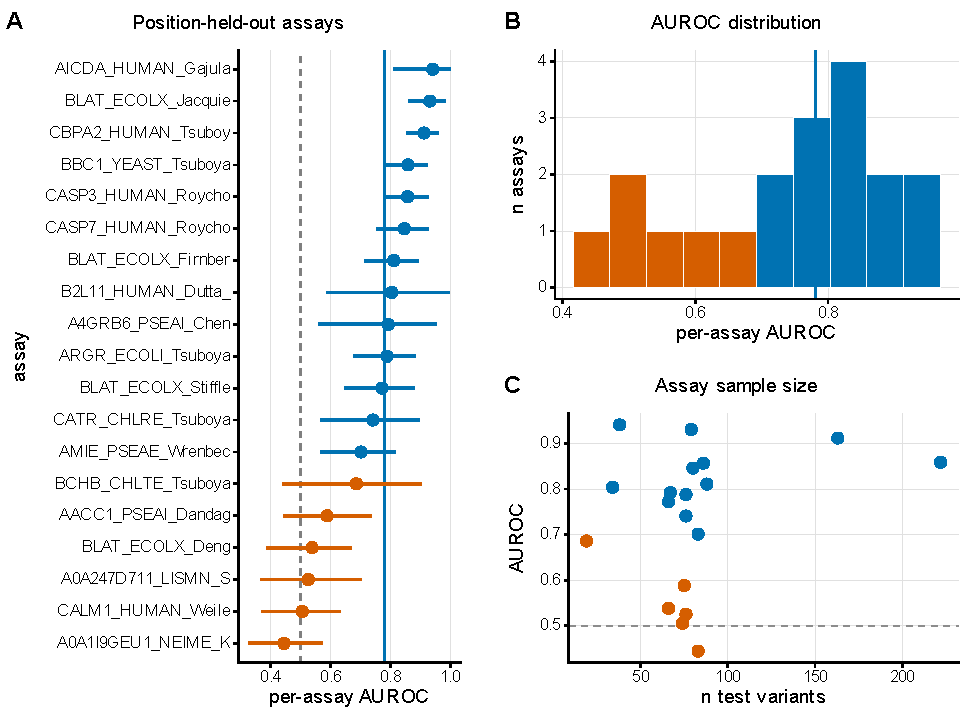
\includegraphics[width=\linewidth,height=0.70\textheight,keepaspectratio]{figures/FS1_proteingym_atlas.pdf}
\caption{{\bf Fig S1. Position-held-out ProteinGym calibration subset.} (A) AUROC and saved 95\% intervals for 19 assays (1,551 test variants); blue indicates intervals excluding chance and orange those including chance. The solid reference is pooled AUROC 0.781 and the dashed reference is chance. (B) Distribution of assay AUROCs. (C) AUROC versus test-set size. Thirteen of 19 assay intervals exclude chance (fraction 0.684211). These are the same assay observations across panels, not independent replications. This position-held-out subset is distinct from the 69-protein scale panel and full 173-protein benchmark. Assay-level exposure labels are unavailable, so neither pretraining-exposure sensitivity nor external transport is established.}

\end{figure}

\begin{figure}[!htbp]
\centering
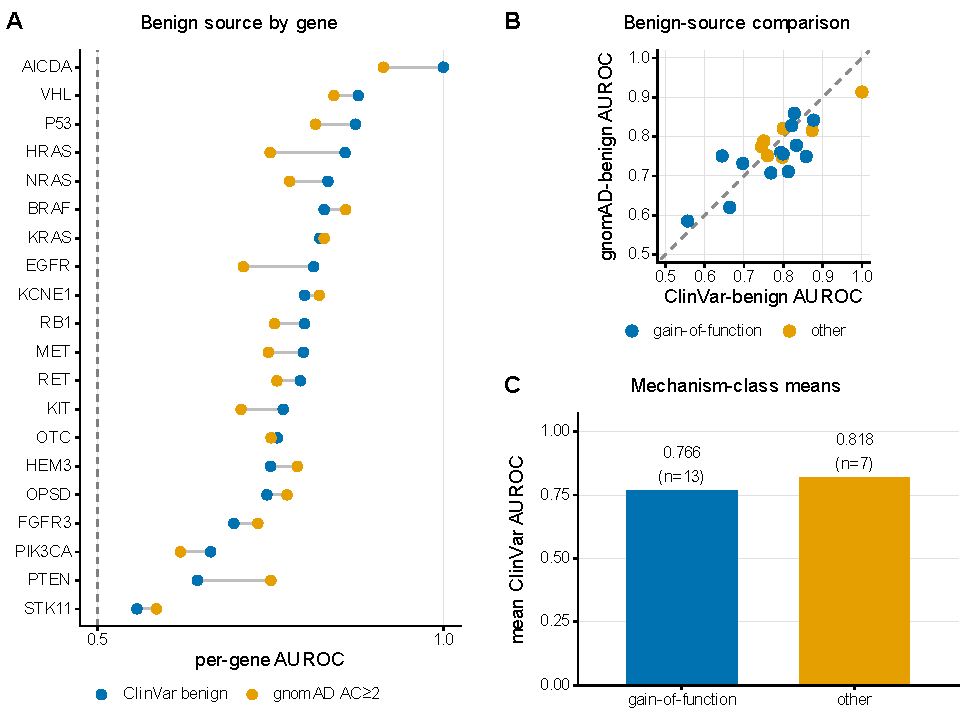
\includegraphics[width=\linewidth,height=0.70\textheight,keepaspectratio]{figures/FS2_gnomad_control.pdf}
\caption{{\bf Fig S2. Historical benign-source sensitivity within the clinical gene panel.} (A) Saved paired per-gene AUROCs using ClinVar-benign and gnomAD allele-count-at-least-two variants, linked on the same scale. All 20 gene names are retained. (B) The same observations on equal axes, coloured by gain-of-function versus other mechanism class. (C) Saved class-mean ClinVar AUROC with gene counts. The saved mean gnomAD-minus-ClinVar difference is $-0.019565$; the other-minus-gain-of-function class-mean difference is 0.0522. Neither aggregate difference has a resampling interval. The gnomAD variants were not rescored in the current revision. These summary-level comparisons do not identify ascertainment effects causally or establish transport to unseen genes.}

\end{figure}

\begin{figure}[!htbp]
\centering
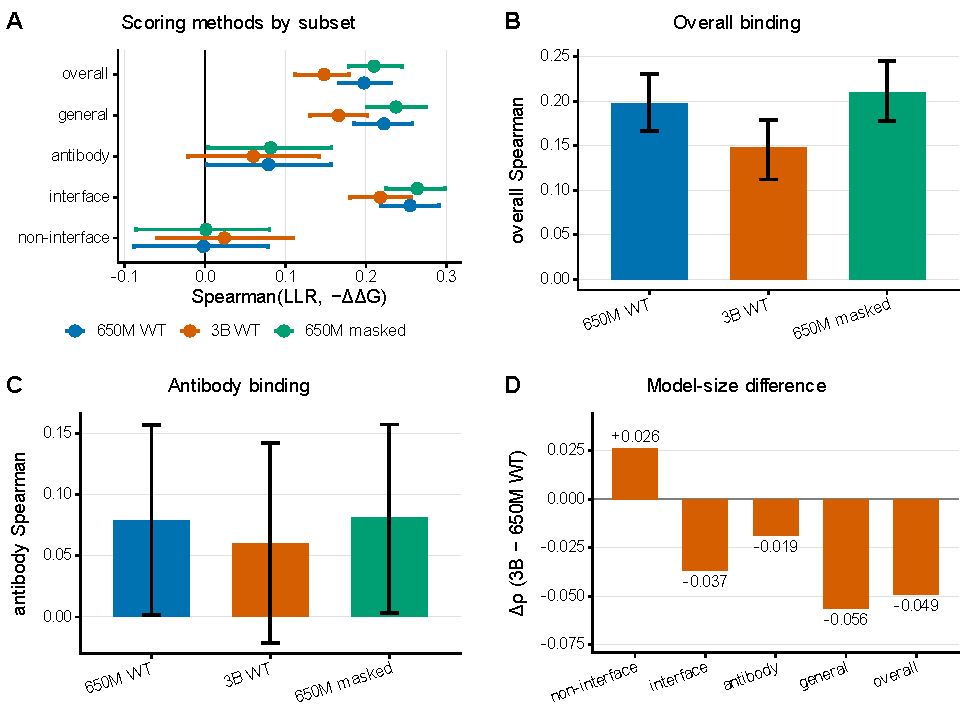
\includegraphics[width=\linewidth,height=0.70\textheight,keepaspectratio]{figures/FS3_antibody_robustness.pdf}
\caption{{\bf Fig S3. Binding sensitivity to model size and scoring convention.} (A) Spearman correlations and saved bootstrap intervals for each SKEMPI subset under 650M WT, 3B WT and 650M masked scoring. (B) Overall binding correlations. (C) Antibody--antigen correlations. (D) The 3B-minus-650M WT difference by subset. All panels reuse 3,424 mutation records with overlapping subset definitions. The saved mean difference across five subsets is $-0.0270622079$; this is not an independent five-experiment estimate. The antibody readout remains weak within these intervals. Missing binding-row coordinates prevent a fresh row-level influence or protein-block-bootstrap analysis; the displayed aggregate intervals do not resolve those limitations.}

\end{figure}

\begin{figure}[!htbp]
\centering
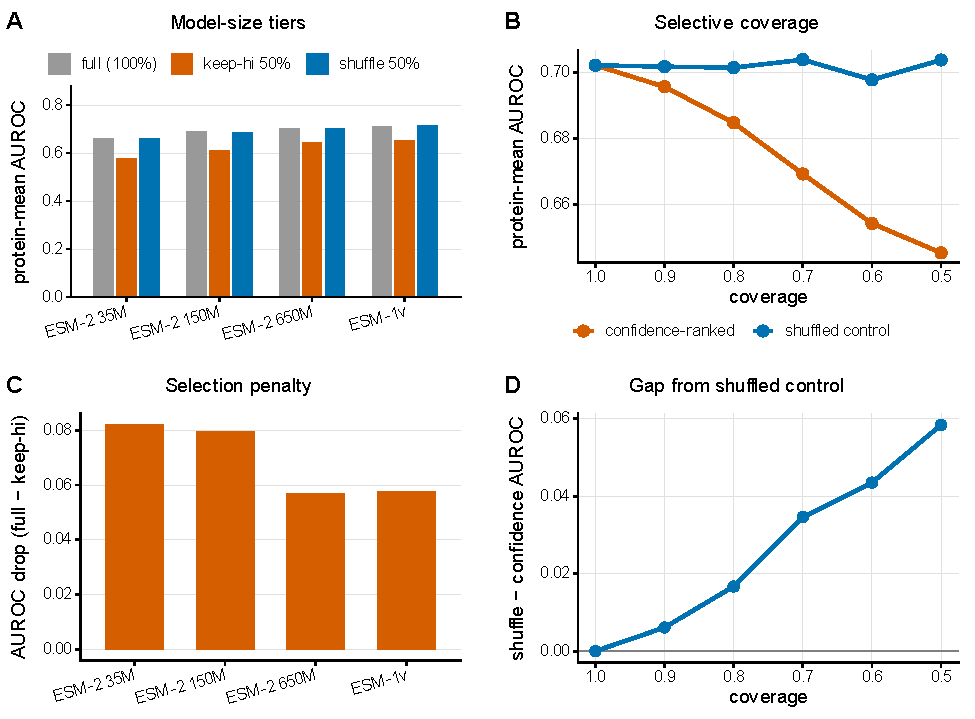
\includegraphics[width=\linewidth,height=0.70\textheight,keepaspectratio]{figures/FS4_abstention_tiers.pdf}
\caption{{\bf Fig S4. Selective ranking by clamped confidence.} (A) Protein-mean AUROC at full coverage, highest-confidence 50\% and a shuffled 50\% control for four model sizes. The common colour legend identifies these conditions. (B) Saved coverage curves for ESM-2 650M. (C) Full-minus-selected AUROC for each size. (D) Shuffled-minus-confidence AUROC at each coverage; positive values favour the shuffled control. These plots reuse the saved tier and coverage observations. Per-protein scores are unavailable for tier-specific resampling, and no validated tier interval or deployable abstention policy is inferred.}

\end{figure}

\begin{figure}[!htbp]
\centering
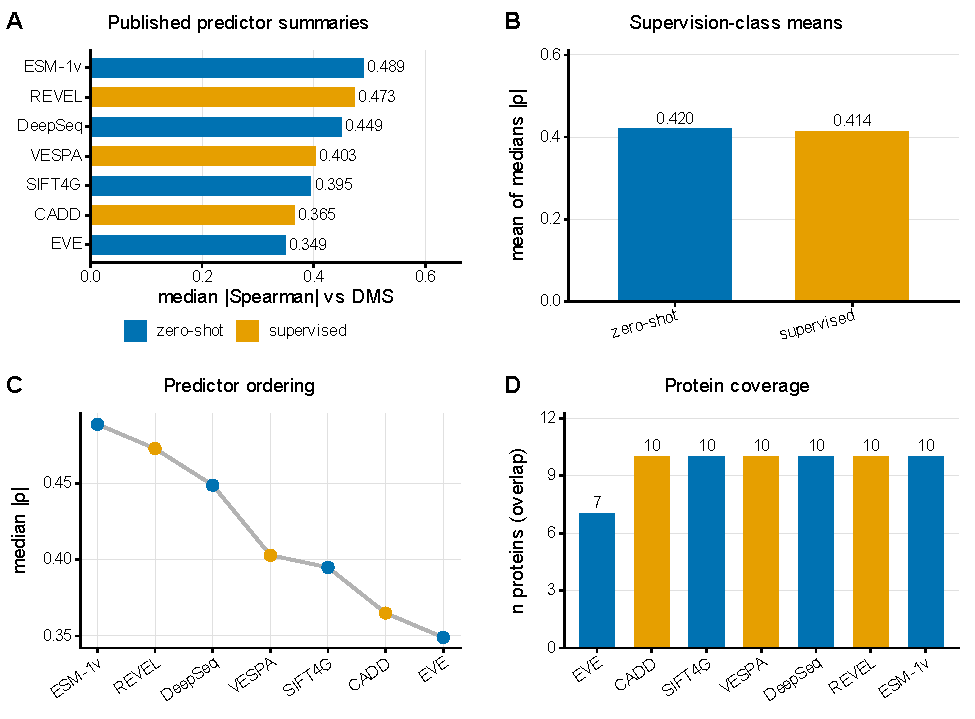
\includegraphics[width=\linewidth,height=0.70\textheight,keepaspectratio]{figures/FS5_vep_comparison.pdf}
\caption{{\bf Fig S5. Published DMS predictor comparisons on a small overlap set.} (A) Median absolute Spearman correlation by predictor. Colours distinguish supervised and zero-shot/unsupervised methods. (B) Saved means of those medians by supervision class. (C) Ordering of the same predictor summaries. (D) Coverage: EVE uses seven proteins and the remaining predictors ten. The saved summary range is 0.14; no interval is available for that range or the class means. Unequal coverage limits direct comparison. These descriptive views reuse the same seven predictor rows and do not establish a universal ranking or an independent performance effect.}

\end{figure}

\begin{figure}[!htbp]
\centering
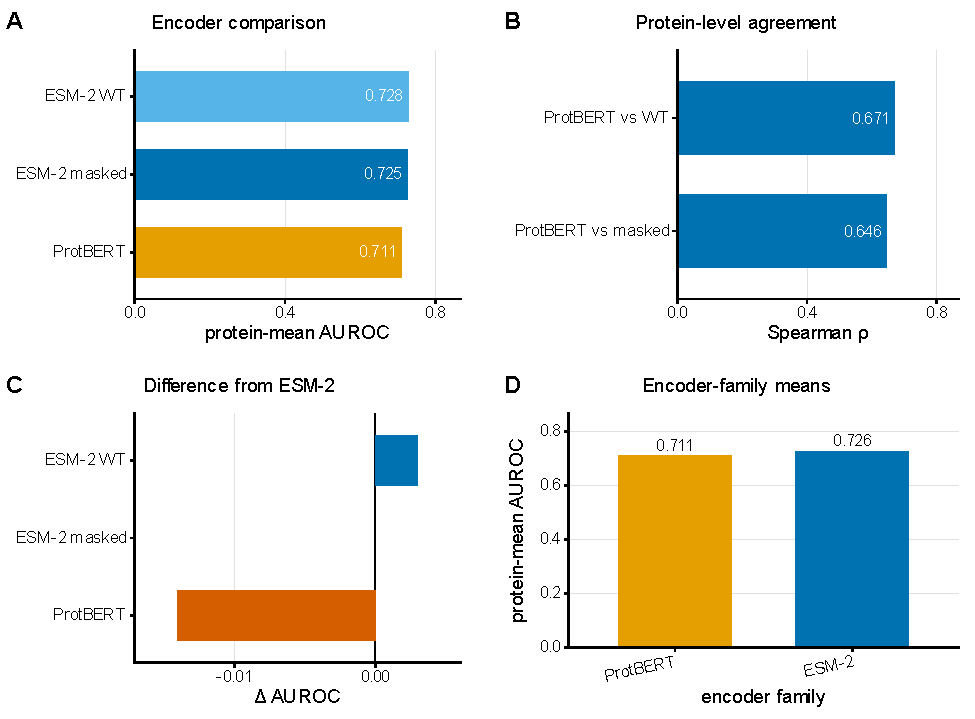
\includegraphics[width=\linewidth,height=0.70\textheight,keepaspectratio]{figures/F2_cross_model.pdf}
\caption{{\bf Fig S6. Cross-encoder discrimination and agreement.} (A) Protein-mean AUROC for ProtBERT and ESM-2 650M under masked- and WT-marginal scoring. (B) Per-protein Spearman agreement between ProtBERT and each ESM-2 scoring convention. (C) AUROC differences relative to ESM-2 masked scoring. (D) Saved encoder-family means. These are aggregate views of the same 69-protein comparison. The saved model-summary range is 0.017 and WT-minus-masked agreement difference 0.025; neither aggregate contrast has a paired interval. The comparison covers masked-language-model encoders and does not evaluate autoregressive or structure-conditioned models.}

\end{figure}

\begin{figure}[!htbp]
\centering
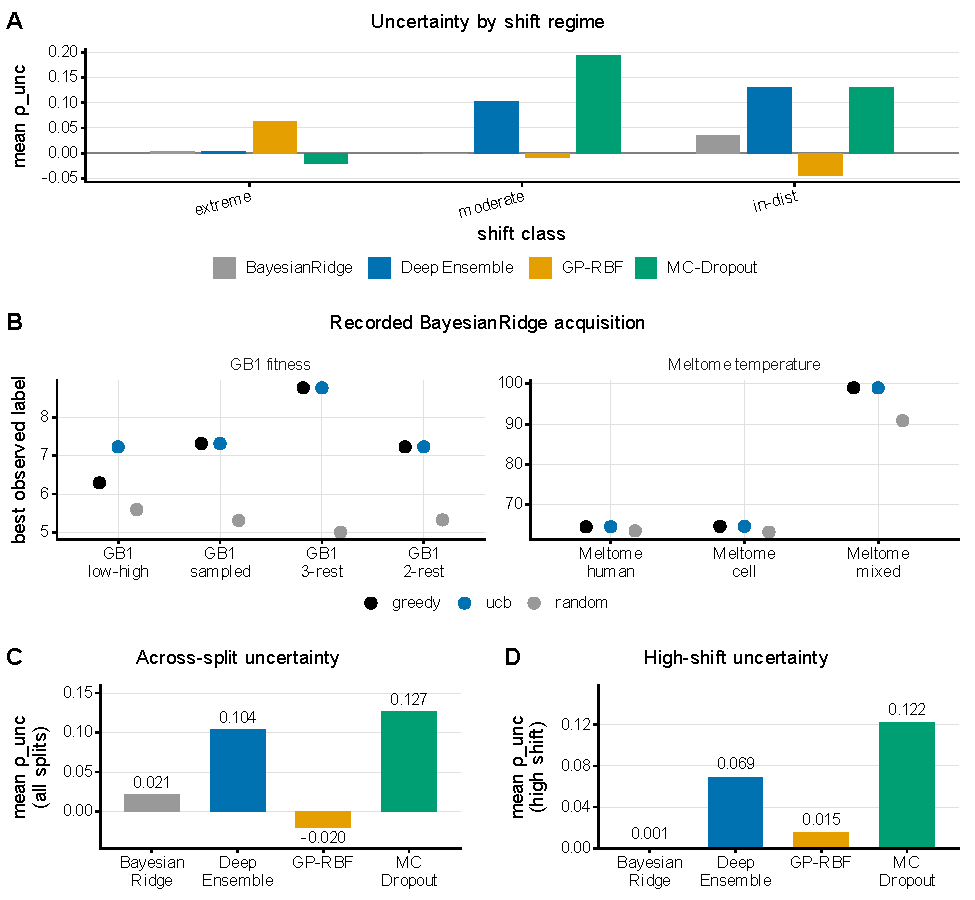
\includegraphics[width=\linewidth,height=0.70\textheight,keepaspectratio]{figures/F6_protein_uq.pdf}
\caption{{\bf Fig S7. Uncertainty and retrospective acquisition retain their source and units.} (A) Saved mean uncertainty--error rank association by shift class and method. (B) BayesianRidge final-best labelled candidates for greedy, UCB and random acquisition. GB1 fitness and Meltome temperature use separate axes and are not averaged across datasets. On GB1 low-versus-high, UCB is 7.2287 and greedy 6.2911; the other displayed UCB and greedy values coincide. These records differ from the cache-based zero-win aggregate, which is omitted from the comparison. (C) Saved mean uncertainty association across seven splits. (D) Saved high-shift means for the same four methods. No new fitting or resampling is performed. The plots are retrospective source records, not prospective assay yields or evidence of generally superior acquisition.}

\end{figure}

\begin{figure}[!htbp]
\centering
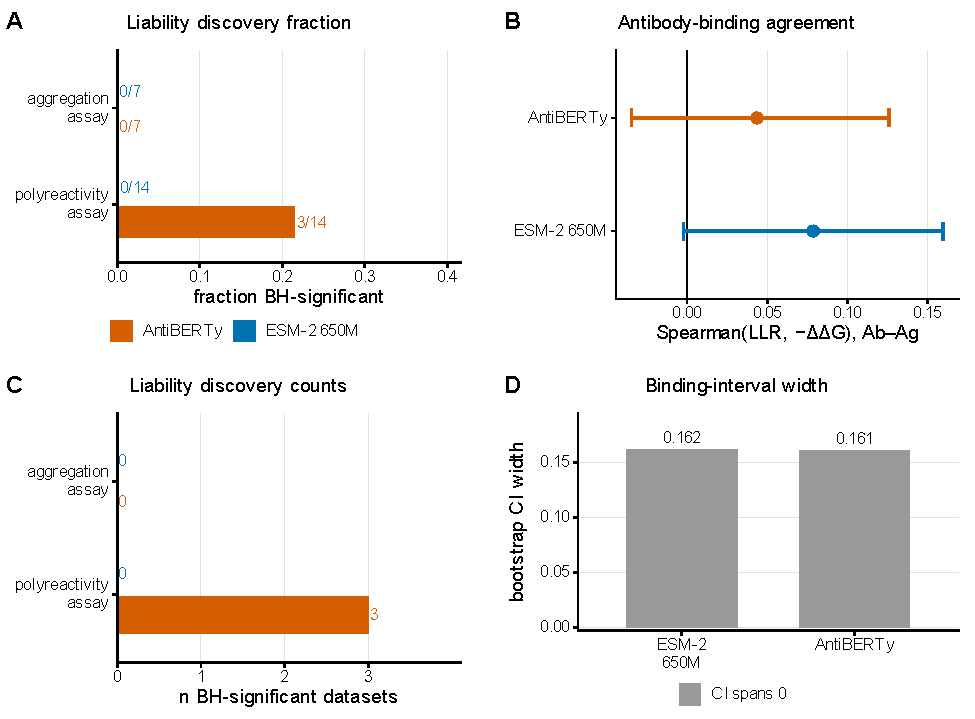
\includegraphics[width=\linewidth,height=0.70\textheight,keepaspectratio]{figures/F9_antibody_lm.pdf}
\caption{{\bf Fig S8. Archived antibody-specific likelihood comparison.} (A) FLAb liability discovery fractions for AntiBERTy and ESM-2, with significant/tested counts including observed zeros. (B) Spearman estimates and intervals preserved from the separate comparison table. Its ESM-2 interval is $[-0.0022,0.1597]$, whereas the N4 summary used in Fig 5 retains $[0.0018,0.1571]$. Similar point estimates do not prove identical rows, scorer or resampling; that provenance remains unresolved. (C) Significant-dataset counts. (D) Widths of the archived intervals, not a new significance comparison. AntiBERTy detects three of fourteen polyreactivity datasets, while neither model detects a BH-significant aggregation association in seven datasets. The saved binding point-estimate difference is 0.0352 and the discovery-count difference is three, without paired uncertainty. The BH family is inherited from the original analysis. These summaries do not establish clinical, mechanistic or deployment validity.}

\end{figure}

\begin{figure}[!htbp]
\centering
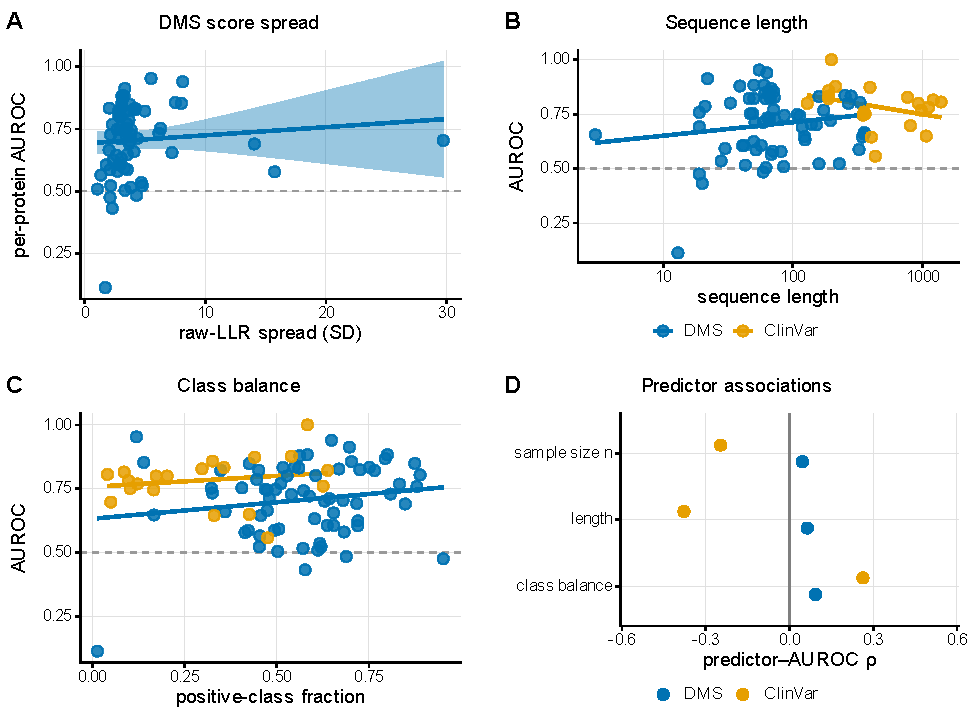
\includegraphics[width=\linewidth,height=0.70\textheight,keepaspectratio]{figures/F10_reliability_predictor.pdf}
\caption{{\bf Fig S9. Exploratory reliability descriptors from the historical predictor table.} (A) DMS AUROC versus raw-LLR spread. (B) AUROC versus sequence length. (C) AUROC versus positive-class fraction. (D) Saved-table predictor associations, with DMS and ClinVar shown separately. The panel contains 69 DMS and 20 clinical summary records; one length is absent and all 69 DMS lengths are proxies. Clinical score spread was absent for all 20 genes: cross-axis transfer of that descriptor was not tested. The historical DMS multivariable fit used sample size, score mean, score standard deviation and length, not class balance. The plots do not establish a transferable predictor, a biological mechanism or failure of an unmeasured descriptor.}

\end{figure}


\clearpage
\section{Same-score clinical analysis}
\begin{table}[!htbp]
\centering\small
\begin{tabular}{lrrrr}
\toprule
Map & ECE & Brier & Log loss & Brier refit range \\
\midrule
Sigmoid($z$) & 0.2563 & 0.2079 & 0.6136 & [0.2038, 0.2120] \\
Platt & 0.0211 & 0.1412 & 0.4441 & [0.1370, 0.1454] \\
Isotonic & 0.0083 & 0.1407 & 0.4445 & [0.1369, 0.1457] \\
Pooled prevalence & 0.0000 & 0.1808 & 0.5475 & [0.1808, 0.1809] \\
Gene prevalence & 0.0100 & 0.1517 & 0.4657 & [0.1518, 0.1540] \\
\bottomrule
\end{tabular}

\caption{{\bf Table S1. Five-fold clinical probability scores.} All point
estimates use 4,677 out-of-fold predictions from the recovered N6c-compatible
LLRs. Brier refit ranges are the 2.5th--97.5th percentiles of 1,000
identity-grouped, gene-by-class-stratified refitting draws. They are not
intervals centred on the fixed-fold point and need not contain it.
The near-zero ECE of pooled prevalence is not evidence of useful variant
discrimination. Gene and class composition are fixed by the resampling
design; no clinical-transport inference is made.}
\end{table}

\begin{table}[!htbp]
\centering\small
\begin{tabular}{lrrr}
\toprule
Map & OOF ECE & Refit mean & Refit percentile range \\
\midrule
Platt & 0.0211 & 0.0247 & [0.0165, 0.0335] \\
Isotonic & 0.0083 & 0.0159 & [0.0090, 0.0253] \\
\bottomrule
\end{tabular}
\caption{{\bf Table S2. Original OOF estimates and refitting distributions.}
These quantities are reported separately to expose resampling and refitting
shifts, not adjusted to reproduce an earlier calibration value. First- and
second-half Platt ECE ranges are [0.0160, 0.0333] and [0.0168, 0.0337];
isotonic ranges are [0.0090, 0.0243] and [0.0090, 0.0257]. All draws and
fold-specific OOF predictions are retained in the reproducibility data.}
\end{table}

The recovered table contains 1,108 pathogenic and 3,569 benign variants.
Per-gene discrimination, per-gene calibration and all reliability-bin
coordinates are separately exported. Historical clinical intervals,
six-gene calibration, Cox/Holm conclusions and degradation counts are not
reused as current evidence. The pooled calibrators use gene-mixed fitting
folds, so the corrected experiment tests within-panel calibration only.
\end{document}
